
% This LaTeX was auto-generated from MATLAB code.
% To make changes, update the MATLAB code and republish this document.

\documentclass{article}
\usepackage{graphicx}
\usepackage{color}

\sloppy
\definecolor{lightgray}{gray}{0.5}
\setlength{\parindent}{0pt}

\begin{document}

    
    

\section*{18. Polynomial roots and colleague matrices}

\begin{verbatim}
ATAPformats
\end{verbatim}
\begin{par}
It is well known that if $p$ is a polynomial expressed as a linear combination of monomials $x^k$, then the roots of $p$ are equal to the eigenvalues of a certain \textit{companion matrix} formed from its coefficients (Exercise 18.1).  Indeed, from its beginning in the late 1970s, Matlab has included a command \texttt{roots} that calculates roots of polynomials by using this identity. This method of zerofinding is effective and numerically stable, but only in a very narrow sense. It is a numerically stable algorithm for precisely the problem just posed: given the monomial coefficients, find the roots.  The trouble is, this problem is an awful one!  As Wilkinson made famous beginning in the 1960s, it is a highly ill-conditioned problem in general [Wilkinson 1984]. The roots tend to be so sensitive to perturbations in the coefficients that even though the algorithm is stable in the sense that it usually produces roots that are exactly correct for a polynomial whose coefficients match the specified ones to a relative error on the order of machine precision [Goedecker 1994, Toh \& Trefethen 1994], this slight perturbation is enough to cause terrible inaccuracy.
\end{par} \vspace{1em}
\begin{par}
There is an exception to this dire state of affairs. Finding roots from polynomial coefficients is a well-conditioned problem in the special case of polynomials with roots on or near the unit circle (see Exercise 18.7(a) and [Sitton, Burrus, Fox \& Treitel 2003]). The trouble is, most applications are not of this kind. More often, the roots of interest lie in or near a real interval, and in such cases one should avoid monomials, companion matrices, and Matlab's \texttt{roots} command completely.
\end{par} \vspace{1em}
\begin{par}

Fortunately, there is a well-conditioned alternative for such problems,
and that is the subject of this chapter. By now we are experts in
working with functions on $[-1,1]$ by means of Chebyshev interpolants and
Chebyshev series. Within this class of tools, there is a natural way of
computing the roots of a polynomial by solving an eigenvalue problem.
Here is the crucial result, due independently to Specht
[1960, p.~222] and Good [1961].\footnote{Jack Good (1916--2009)
was a hero of Bayesianism who worked with Turing at Bletchley
Park.}  The matrix $C$ of the theorem is called a {\em colleague matrix}.

\end{par} \vspace{1em}
\begin{par}
\textbf{Theorem 18.1. Polynomial roots and colleague matrix eigenvalues.} \textit{The roots of the polynomial} $$ p(x) = \sum_{k=0}^n  a_k T_k(x),\quad a_n \ne 0 $$ \textit{are the eigenvalues of the matrix} $$ C = \pmatrix{0&1\cr\noalign{\vskip 4pt} {1\over 2}&0&{1\over 2} \cr \noalign{\vskip 4pt} &{1\over 2}&0&{1\over 2}\cr\noalign{\vskip 4pt} &&\ddots&\ddots&\ddots\cr\noalign{\vskip 2pt} &&&&&{1\over 2}\cr\noalign{\vskip 4pt} &&&&{1\over 2}&0} - {1\over 2 a_n} \pmatrix{~~\cr\noalign{\vskip 78pt} a_0 & a_1 & a_2 & \dots & a_{n-1}}. \eqno (18.1) $$ (\textit{Entries not displayed are zero.)  If there are multiple roots, these correspond to eigenvalues with the same multiplicities.}
\end{par} \vspace{1em}
\begin{par}
\textit{Proof.}  Let $x$ be any number, and consider the nonzero $n$-vector $$ v = (T_0(x), T_1(x), \dots , T_{n-1}(x))^T. $$ If we multiply $C$ by $v$, then in every row but the first and last the result is $$ T_k(x) \mapsto {\textstyle{1\over 2}} T_{k-1}(x) + {\textstyle{1\over 2}} T_{k+1}(x) = x \kern 1pt T_k(x), $$ thanks to the three-term recurrence relation (3.9) for Chebyshev polynomials.  In the first row we likewise have $$ T_0(x) \mapsto T_1(x) = x \kern 1pt T_0(x) $$ since $T_0(x) = 1$ and $T_1(x) = x$.  It remains to examine the bottom row.  Here it is convenient to imagine that in the difference of matrices defining $C$ above, the ``missing'' entry $1/2$ is added in the $(n,n+1)$ position of the first matrix and subtracted again from the $(n,n+1)$ position of the second matrix.  Then by considering the recurrence relation again we find $$ T_{n-1}(x) \mapsto x\kern 1pt T_{n-1}(x) - {1\over 2a_n} (a_0T_0(x) + a_1 T_1(x) + \cdots + a_n T_n(x)). $$ This equation holds for any $x$, and if $x$ is a root of $p$, then the term in parentheses on the right vanishes.  In other words, if $x$ is a root of $p$, then $Cv$ is equal to $xv$ in every entry, making $v$ is an eigenvector of $C$ with eigenvalue $x$.  If $p$ has $n$ distinct roots, this implies that they are precisely the eigenvalues of $C$, and this completes the proof in the case where $p$ has distinct roots.
\end{par} \vspace{1em}
\begin{par}
If $p$ has multiple roots, we must show that each one corresponds to an eigenvalue of $C$ with the same multiplicity.  For this we can consider perturbations of the coefficients $a_0, \dots, a_{n-1}$ of $p$ with the property that the roots become distinct.  Each root must then correspond to an eigenvalue of the correspondingly perturbed matrix $C$, and since both roots of polynomials and eigenvalues of matrices are continuous functions of the parameters, the multiplicities must be preserved in the limit as the amplitude of the perturbations goes to zero. $~\hbox{\vrule width 2.5pt depth 2.5 pt height 3.5 pt}$
\end{par} \vspace{1em}
\begin{par}
As mentioned above, the matrix $C$ of (18.1) is called a colleague matrix. Theorem 18.1 has been rediscovered several times, for example by Day \& Romero [2005].  Since Specht [1957] there have also been generalizations to other families of orthogonal polynomials besides Chebyshev polynomials, and the associated generalized colleague matrices are called \textit{comrade matrices} [Barnett 1975a \& 1975b]. The generalization is immediate: one need only change the entries of rows $1$ to $n-1$ to correspond to the appropriate recurrence relation.
\end{par} \vspace{1em}
\begin{par}
For an example to illustrate Theorem 18.1, consider the polynomial $p(x) = x(x-1/4)(x-1/2)$.
\end{par} \vspace{1em}
\begin{par}
 \vskip -2em 
\end{par} \vspace{1em}
\begin{verbatim}
x = chebfun('x');
p = x.*(x-1/4).*(x-1/2);
clf, plot(p)
axis([-1 1 -.5 .5]), grid on
set(gca,'xtick',-1:.25:1)
title('A cubic polynomial','fontsize',9)
\end{verbatim}

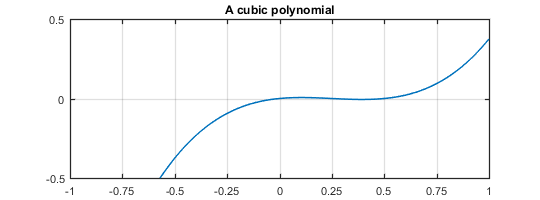
\includegraphics [width=4in]{chap18_01.png}
\begin{par}
 \vskip 1pt

\end{par} \vspace{1em}
\begin{par}
Obviously $p$ has roots 0, 1/4, and 1/2.  The Chebyshev coefficients are $-3/8, 7/8, -3/8, 1/4$:
\end{par} \vspace{1em}
\begin{par}

\vskip -2em

\end{par} \vspace{1em}
\begin{verbatim}
format short
a = fliplr(chebpoly(p))
\end{verbatim}

        \color{lightgray} \begin{verbatim}a =
   -0.3750    0.8750   -0.3750    0.2500
\end{verbatim} \color{black}
    \begin{par}
As expected, the colleague matrix (18.1) for this polynomial,
\end{par} \vspace{1em}
\begin{par}
 \vskip -2em 
\end{par} \vspace{1em}
\begin{verbatim}
C = [0 1 0; 1/2 0 1/2; 0 1/2 0] - ...
    (1/(2*a(4)))*[0 0 0; 0 0 0; a(1:3)]
\end{verbatim}

        \color{lightgray} \begin{verbatim}C =
         0    1.0000         0
    0.5000         0    0.5000
    0.7500   -1.2500    0.7500
\end{verbatim} \color{black}
    \begin{par}
has eigenvalues that match the roots of $p$:
\end{par} \vspace{1em}
\begin{par}
 \vskip -2em 
\end{par} \vspace{1em}
\begin{verbatim}
format long
eig(C)
\end{verbatim}

        \color{lightgray} \begin{verbatim}ans =
                   0
   0.500000000000001
   0.250000000000000
\end{verbatim} \color{black}
    \begin{par}
In Chebfun, every function is represented by a polynomial or a piecewise polynomial.  Theorem 18.1 provides Chebfun with its method of numerical rootfinding, implemented in the Chebfun \texttt{roots} command.  For this polynomial \texttt{p}, we can call \texttt{roots} to add the roots to the plot, like this:
\end{par} \vspace{1em}
\begin{par}
 \vskip -2em 
\end{par} \vspace{1em}
\begin{verbatim}
r = roots(p);
hold on, plot(r,p(r),'or','markersize',7)
title('Roots of the polynomial','fontsize',9)
\end{verbatim}

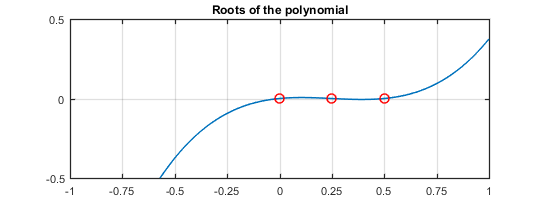
\includegraphics [width=4in]{chap18_02.png}
\begin{par}
 \vskip 1pt 
\end{par} \vspace{1em}
\begin{par}
In this example, \texttt{p} was a polynomial from the start. The real power of Theorem 18.1, however, comes when it is applied to the problem of finding the roots on $[-1,1]$ of a general function $f$. To do this, we first approximate $f$ by a polynomial, then find the roots of the polynomial. This idea was proposed in Good's original 1961 paper [Good 1961]. In a more numerical era, it has been advocated in a number of papers by John Boyd, including [Boyd 2002], and it is exploited virtually every time Chebfun is used.
\end{par} \vspace{1em}
\begin{par}
For example, here is the chebfun corresponding to $\cos(50\pi x)$ on $[-1,1]$:
\end{par} \vspace{1em}
\begin{par}
 \vskip -2em 
\end{par} \vspace{1em}
\begin{verbatim}
f = cos(50*pi*x); length(f)
\end{verbatim}

        \color{lightgray} \begin{verbatim}ans =
   213
\end{verbatim} \color{black}
    \begin{par}
It doesn't take long to compute its roots,
\end{par} \vspace{1em}
\begin{par}
 \vskip -2em 
\end{par} \vspace{1em}
\begin{verbatim}
tic, r = roots(f); toc
\end{verbatim}

        \color{lightgray} \begin{verbatim}Elapsed time is 0.083420 seconds.
\end{verbatim} \color{black}
    \begin{par}
The exact roots of this function on $[-1,1]$ are $-0.99, -0.97,\dots,0.97,0.99$. Inspecting a few of the computed results shows they are accurate to close to machine precision:
\end{par} \vspace{1em}
\begin{par}
 \vskip -2em 
\end{par} \vspace{1em}
\begin{verbatim}
r(1:5)
\end{verbatim}

        \color{lightgray} \begin{verbatim}ans =
  -0.990000000000000
  -0.970000000000000
  -0.950000000000000
  -0.930000000000000
  -0.910000000000000
\end{verbatim} \color{black}
    \begin{par}
Changing the function to $\cos(500\pi x)$ makes the chebfun ten times longer,
\end{par} \vspace{1em}
\begin{par}
 \vskip -2em 
\end{par} \vspace{1em}
\begin{verbatim}
f = cos(500*pi*x); length(f)
\end{verbatim}

        \color{lightgray} \begin{verbatim}ans =
        1685
\end{verbatim} \color{black}
    \begin{par}
One might think this would increase the rootfinding time greatly, since the number of operations for an eigenvalue computation grows with the cube of the matrix dimension.  (The colleague matrix has special structure that can be used to bring the operation count down to $O(n^2)$, but this is not done in a straightforward Matlab call to \texttt{eig}.) However, an experiment shows that the timing is still quite good,
\end{par} \vspace{1em}
\begin{par}
 \vskip -2em 
\end{par} \vspace{1em}
\begin{verbatim}
tic, r = roots(f); toc
\end{verbatim}

        \color{lightgray} \begin{verbatim}Elapsed time is 0.240060 seconds.
\end{verbatim} \color{black}
    \begin{par}
and the accuracy is still outstanding:
\end{par} \vspace{1em}
\begin{par}
 \vskip -2em 
\end{par} \vspace{1em}
\begin{verbatim}
r(1:5)
\end{verbatim}

        \color{lightgray} \begin{verbatim}ans =
  -0.999000000000000
  -0.997000000000000
  -0.995000000000000
  -0.993000000000000
  -0.991000000000000
\end{verbatim} \color{black}
    \begin{par}
We can make sure all 1000 roots are equally accurate by computing a norm:
\end{par} \vspace{1em}
\begin{par}
 \vskip -2em 
\end{par} \vspace{1em}
\begin{verbatim}
exact = [-0.999:0.002:0.999]'; norm(r-exact,inf)
\end{verbatim}

        \color{lightgray} \begin{verbatim}ans =
     3.330669073875470e-16
\end{verbatim} \color{black}
    \begin{par}
The explanation of this great speed in finding the roots of a polynomial of degree in the thousands is that the complexity of the algorithm has been improved from $O(n^3)$ to $O(n^2)$ by recursion. If a chebfun has length greater than 100, the interval is divided recursively into subintervals, with a chebfun constructed on each subinterval of appropriately lower degree. Thus no eigenvalue problem is ever solved of dimension greater than 100. This idea of rootfinding based on recursive subdivision of intervals and Chebyshev eigenvalue problems was developed by John Boyd in the 1980s and 1990s and published by him in 2002 [Boyd 2002].  Details of the original Chebfun implementation of \texttt{roots} were presented in [Battles 2005], and in 2012 the Chebfun algorithm was speeded up substantially by Pedro Gonnet (unpublished).
\end{par} \vspace{1em}
\begin{par}
These techniques are remarkably powerful for practical computations. For example, how many zeros does the Bessel function $J_0$ have in the interval $[0,5000]$?  Chebfun finds the answer in a fraction of a second:
\end{par} \vspace{1em}
\begin{par}
 \vskip -2em 
\end{par} \vspace{1em}
\begin{verbatim}
tic, f = chebfun(@(x) besselj(0,x),[0,5000]);
r = roots(f); toc
length(r)
\end{verbatim}

        \color{lightgray} \begin{verbatim}Elapsed time is 0.485275 seconds.
ans =
        1591
\end{verbatim} \color{black}
    \begin{par}
What is the the 1000th zero?
\end{par} \vspace{1em}
\begin{par}
 \vskip -2em 
\end{par} \vspace{1em}
\begin{verbatim}
r(1000)
\end{verbatim}

        \color{lightgray} \begin{verbatim}ans =
     3.140807295225079e+03
\end{verbatim} \color{black}
    \begin{par}
We readily verify that this zero is an accurate one:
\end{par} \vspace{1em}
\begin{par}
 \vskip -2em 
\end{par} \vspace{1em}
\begin{verbatim}
besselj(0,ans)
\end{verbatim}

        \color{lightgray} \begin{verbatim}ans =
     5.756205180307391e-17
\end{verbatim} \color{black}
    \begin{par}
This example, like a few others scattered around the book, makes use of a chebfun defined on an interval other than the default $[-1,1]$.  The mathematics is straightforward; $[0,5000]$ is reduced to $[-1,1]$ by a linear transformation.
\end{par} \vspace{1em}
\begin{par}

Here is another illustration of recursive colleague matrix rootfinding for
a high-order polynomial.  The function
$$ f(x) = e^x[\hbox{sech}(4 \sin(40x))]^{\exp(x)} \eqno (18.1) $$
features a row of narrower and narrower spikes.  Where in $[-1,1]$
does it take the value $1$? We can find the answer by using {\tt roots}
to find the zeros of the equation $f(x)-1=0$:

\end{par} \vspace{1em}
\begin{par}
 \vskip -2em 
\end{par} \vspace{1em}
\begin{verbatim}
ff = @(x) exp(x).*sech(4*sin(40*x)).^exp(x);
tic, f = ff(x); r = roots(f-1); toc
clf, plot(f), grid on, FS = 'fontsize';
title('Return to the challenging integrand (18.14)',FS,9)
hold on, plot(r,f(r),'or','markersize',4)
\end{verbatim}

        \color{lightgray} \begin{verbatim}Elapsed time is 0.366501 seconds.
\end{verbatim} \color{black}
    
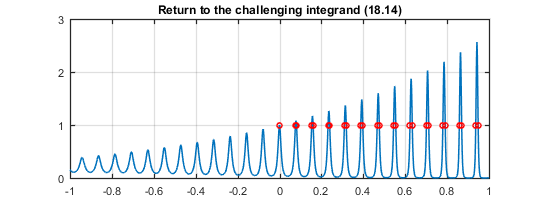
\includegraphics [width=4in]{chap18_03.png}
\begin{par}
 \vskip 1pt 
\end{par} \vspace{1em}
\begin{par}
Notice that we have found the roots here of a polynomial of quite high degree:
\end{par} \vspace{1em}
\begin{par}
 \vskip -2em 
\end{par} \vspace{1em}
\begin{verbatim}
length(f)
\end{verbatim}

        \color{lightgray} \begin{verbatim}ans =
        3680
\end{verbatim} \color{black}
    \begin{par}
A numerical check confirms that the roots are accurate,
\end{par} \vspace{1em}
\begin{par}
 \vskip -2em 
\end{par} \vspace{1em}
\begin{verbatim}
max(abs(ff(r)-1))
\end{verbatim}

        \color{lightgray} \begin{verbatim}ans =
     6.172840016915870e-14
\end{verbatim} \color{black}
    \begin{par}
and zooming in gives perhaps a more convincing plot:
\end{par} \vspace{1em}
\begin{par}
 \vskip -2em 
\end{par} \vspace{1em}
\begin{verbatim}
xlim([-.1 .27])
title('Close-up',FS,9)
\end{verbatim}

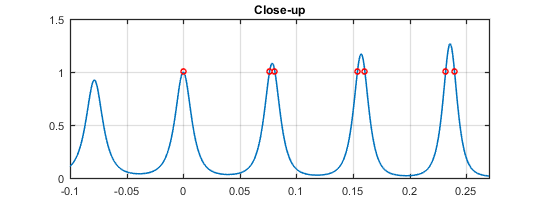
\includegraphics [width=4in]{chap18_04.png}
\begin{par}
 \vskip 1pt 
\end{par} \vspace{1em}
\begin{par}
Computations like this are examples of \textit{global rootfinding}, a special case of \textit{global optimization}.  They are made possible by the combination of fast methods of polynomial approximation with the extraordinarily fast and accurate methods for matrix eigenvalue problems that have been developed in the years since Francis invented the QR algorithm in the very same year as Good proposed his colleague matrices [Francis 1961]. (A crucial algorithmic feature that makes these eigenvalue calculations so accurate is known as ``balancing'', introduced in [Parlett \& Reinsch 1969]---see [Toh \& Trefethen 1994] and Exercise 18.3.)
\end{par} \vspace{1em}
\begin{par}
Global rootfinding is a step in many other practical computations. It is used by Chebfun, for example, in computing minima, maxima, $1$-norms, and absolute values.
\end{par} \vspace{1em}
\begin{par}
 It is worth mentioning that as an alternative to eigenvalue
problems based on Chebyshev expansion coefficients, it is possible to
relate roots of polynomials to eigenvalue problems (or generalized
eigenvalue problems) constructed from function values themselves at
Chebyshev or other points.  Mathematical processes along these lines are
described in [Fortune 2001], [Amiraslani, et al.\ 2004], and
[Amiraslani 2006].  So far there
has not been much numerical exploitation of these ideas, but preliminary
experiments suggest that in the long run they may be competitive.

\end{par} \vspace{1em}
\begin{par}
We close this chapter by clarifying a point that may have puzzled the reader, and which has fascinating theoretical connections. In plots like the last two, we see only real roots of a function.  Yet if the function is a chebfun based on a polynomial representation, won't there be complex roots too? This is indeed the case, but the Chebfun \texttt{roots} command by default returns only those roots in the interval where the function is defined. This default behavior can be overridden by the use of the flags \texttt{'all'} or \texttt{'complex'} (see Exercise 14.2). For example, suppose we make a chebfun corresponding to the function $f(x) = (x-0.5)/(1+10x^2)$, which has just one root in the complex plane, at $x=0.5$:
\end{par} \vspace{1em}
\begin{par}
 \vskip -2em 
\end{par} \vspace{1em}
\begin{verbatim}
f = (x-0.5)./(1+10*x.^2); length(f)
\end{verbatim}

        \color{lightgray} \begin{verbatim}ans =
   119
\end{verbatim} \color{black}
    \begin{par}
Typing \texttt{roots} alone gives just the root at $x=0.5$:
\end{par} \vspace{1em}
\begin{par}
 \vskip -2em 
\end{par} \vspace{1em}
\begin{verbatim}
roots(f)
\end{verbatim}

        \color{lightgray} \begin{verbatim}ans =
   0.499999999999999
\end{verbatim} \color{black}
    \begin{par}
With \texttt{roots(f,'all')}, however, we get 106 roots:
\end{par} \vspace{1em}
\begin{par}
 \vskip -2em 
\end{par} \vspace{1em}
\begin{verbatim}
r = roots(f,'all'); length(r)
\end{verbatim}

        \color{lightgray} \begin{verbatim}ans =
   112
\end{verbatim} \color{black}
    \begin{par}

The complex roots are meaningless from the point of view of the underlying
function $f$; they are an epiphenomenon that arises in the process of
approximating $f$ on $[-1,1]$. A plot reveals that they have a familiar
distribution, lying almost exactly on the Chebfun ellipse for this function:

\end{par} \vspace{1em}
\begin{par}
 \vskip -2em 
\end{par} \vspace{1em}
\begin{verbatim}
hold off, chebellipseplot(f,'r')
hold on, plot(r,'.','markersize',10)
xlim(1.2*[-1 1]), grid on, axis equal
FS = 'fontsize';
title('Illustration of the theorem of Walsh',FS,9)
\end{verbatim}

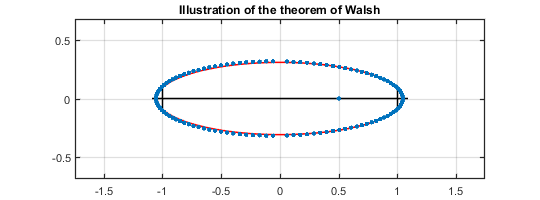
\includegraphics [width=4in]{chap18_05.png}
\begin{par}
 \vspace{1pt} 
\end{par} \vspace{1em}
\begin{par}
The fact that roots of best and near-best approximations cluster along the maximum Bernstein ellipse of analyticity is a special case of a theorem due to Walsh [1959]. Blatt and Saff [1986] extended Walsh's result to the case in which the function being approximated has no ellipse of analyticity, but is merely continuous on $[-1,1]$. They showed that in this case, the zeros of the best approximants always cluster at every point of the interval as $n\to\infty$.  This phenomenon applies not only to the best approximations, but to all near-best best approximations that are maximally convergent as defined in Chapter 12, hence in particular to Chebyshev interpolants. Here for example are the roots of the degree 100 Chebyshev interpolant to $|x|$:
\end{par} \vspace{1em}
\begin{par}
 \vskip -2em 
\end{par} \vspace{1em}
\begin{verbatim}
f = chebfun('abs(x)',101); length(f)
r = roots(f,'all');
hold off, plot([-1,1],[0,0],'r')
hold on, plot(r,'.','markersize',10)
xlim(1.2*[-1 1]), grid on, axis equal
title('Illustration of the theorem of Blatt and Saff',FS,9)
\end{verbatim}

        \color{lightgray} \begin{verbatim}ans =
   101
\end{verbatim} \color{black}
    
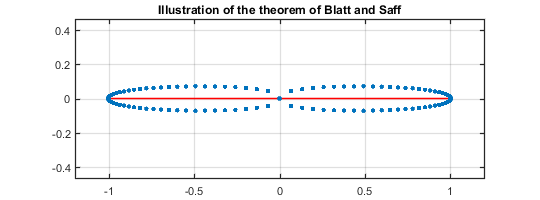
\includegraphics [width=4in]{chap18_06.png}
\begin{par}
 \vskip 1pt 
\end{par} \vspace{1em}
\begin{par}
The Walsh and Blatt--Saff theorems are extensions of \textit{Jentzsch's theorem}, which asserts that the partial sums of Taylor series have roots clustering along every point of the circle of convergence [Jentzsch 1914].
\end{par} \vspace{1em}
\begin{par}

\begin{displaymath}
\framebox[4.7in][c]{\parbox{4.5in}{\vspace{2pt}\sl
{\sc Summary of Chapter 18.}
The roots of a polynomial are equal to the eigenvalues of a colleague
matrix formed from its coefficients in a Chebyshev series, tridiagonal
except in the final row. This identity, combined
with recursive subdivision, leads to a stable and efficient numerical
method for computing roots of a polynomial in an interval.  For
orthogonal polynomials other than Chebyshev, the colleague matrix
generalizes to a comrade matrix with the same almost-tridiagonal
structure.\vspace{2pt}}}
\end{displaymath}

\end{par} \vspace{1em}
\begin{par}
 \small\smallskip\parskip=2pt
\par
{\bf Exercise 18.1.  Companion matrix.}  Prove that the roots of the
polynomial $p(x) = a_0 + a_1x + \cdots + a_n x^n$, $a_n\ne 0$, are the
eigenvalues of the $n\times n$ matrix with zero
entries everywhere except for the value $1$ in the first superdiagonal
and the values $-a_0/a_n,\dots,-a_{n-1}/a_n$ in the last row.
\par
{\bf Exercise 18.2.  Four forms of colleague matrix.}
A matrix $C$ has the same eigenvalues and eigenvalue multiplicities as
$C^T$ and also as $SCS^{-1}$, where $S$ is any nonsingular matrix.  Use
these properties to derive three alternative forms of the colleague
matrix in which the Chebyshev coefficients appear in (a) the first row,
(b) the first column, (c) the last column.
\par
{\bf Exercise 18.3.  Some forms more stable than others.}
Mathematically, all the matrices described in the last exercise have the
same eigenvalues.  Numerically, however, some may suffer more than others
from rounding errors, and in fact Chebfun works with the first-column
option for just this reason. (a) Determine the $11\times 11$ colleague
matrix corresponding to roots $-1, -0.8, -0.6, \dots, 1$.  Get the
entries of the matrix exactly, either analytically or by intelligent
guesswork based on Matlab's \verb|rat| command.
(b) How does the accuracy of the
eigenvalues of the four matrix variants compare?  Which one is best?
Is the difference significant?  (c) What happens if you solve the
four eigenvalue problems again using Matlab's \verb|'nobalance'| option
in the \verb|eig| command?
\par
{\bf Exercise 18.4. Legendre polynomials.}  The Legendre
polynomials satisfy $P_0(x) = 1$, $P_1(x) = x$, and for
$k\ge 1$, the recurrence relation (17.6).
(a) Derive a ``comrade matrix'' analogue of Theorem 18.1 for the roots
of a polynomial expanded as a linear combination of Legendre polynomials.
(b) Verify numerically that the roots of the particular polynomial $P_0 +
P_1 + \cdots + P_5$ match the prediction of your theorem.  (Try
\verb|sum(legpoly(0:5),2)| to construct this polynomial elegantly in
Chebfun and don't forget \verb|roots(...,'all')|.)
\par
{\bf Exercise 18.5.  Complex roots.}  For each of the following functions
defined on $[-1,1]$, construct corresponding chebfuns and plot
all their roots in the complex plane with
\verb|plot(roots(f,'all'))|.  Comment on the patterns you observe.
(Your comments are not expected to go very deep.)
(a) $x^{20}-1$,
(b) $\exp(x)(x^{20}-1)$,
(c) $1/(1+25x^2)$,
(d) $x\exp(30ix)$,
(e) $\sin(10\pi x)$,
(f) $\sqrt{1.1-x}$,
(g) An example of your own choosing.
\par
{\bf Exercise 18.6.  The Szeg\H o curve.}  If $f$ is entire,
then it has no maximal Bernstein ellipse of analyticity.
Plot the roots in
the complex $x$-plane of the Chebfun polynomial approximation to $e^x$ on
$[-1,1]$, and for comparison, the ``Szeg\H o curve'' defined by
$|x\kern .7pt e^{1-x}|=1$ and $|x|\le 1$
[Szeg\H o 1924, Saff \& Varga 1978b, Pritsker \& Varga 1997].
\par
{\bf Exercise 18.7.  Roots of random polynomials.}  (a) Use Matlab's
\verb|roots| command to plot the roots of a polynomial
$p(z) = a_0^{}+a_1^{}z + \cdots + a_{200}^{}z^{200}$
with coefficients selected from the standard normal distribution.
(b) Use \verb|chebfun('randn(201,1)','coeffs')| and
\verb|plot(roots(p,'all'))| to plot the roots of a polynomial
$p(x) = a_0^{}T_0+a_1^{}T_1(x) + \cdots + a_{200}^{}T_{200}(x)$ with the
same kind of random coefficients.
(Effects like these are analyzed rigorously in [Shiffman \& Zelditch 2003].)
\par 
\end{par} \vspace{1em}



\end{document}
    
